% \lipsum[2-3]

\section{Motivation}
\section{Aufgabenstellung}
\section{Zusammenfassung des Projektergebnisse}
\setauthor{Arsham Edalatkhah}

\begin{itemize}
    \item \textbf{Auszeichnungen:}
    \begin{itemize}
        \item \textbf{\#1 Platz Linz hACkT Event X Innovationshauptplatz}
        \item \textbf{\#1 Platz mPreneur Austria Contest X ICT4D.at}
        \item \textbf{\#1 Platz Immotopia Innovation Award}
        \item \textbf{\#3 Platz Spusu Innovation Award (Austria - Wien)}
        \item \textbf{Sieger Team bei mPreneur School Ohrid X World Summit Award}
        \item \textbf{Projekt-Präsentation für den Linzer Bürgermeister und Magistrasdirektorin}
    \end{itemize}
    \item \textbf{Teilnahme an Workshops:}
    \begin{itemize}
        \item \textbf{Workshop Planet Linz Days}
        \item \textbf{Workshop Jugendhackt Österreich}
        \item \textbf{Workshop Project-Forge ICT4D.at}
    \end{itemize}
    \item \textbf{Workshops, die der Arsham Edalatkhah im Rahmen der Diplomarbeit gehostet hat:}
    \begin{itemize}
        \item \textbf{Workshop Präsentationstechnik an der HTL Leonding}
        \item \textbf{Workshop Radio-Training an der HTL Leonding}
    \end{itemize}
    \item \textbf{Medienauftritte:}
    \begin{itemize}
        \item \textbf{Oberösterreicher des Tages (Arsham Edalatkhah)}
        \item \textbf{UNESCO Internet4trust Konferenz}
    \end{itemize}
    \item \textbf{Bevorstehende Events:}
    \begin{itemize}
        \item \textbf{World Summit Award (Austria - Graz)}
        \item \textbf{Project Awards an der HTL Leonding}
    \end{itemize}
\end{itemize}

Seit Beginn unseres Diplomarbeitsprojekts konzentrierte sich das Nochba Team auf die Entwicklung einer App, die sich auf soziale Aspekte im Bereich des Ressourcen-Sharings und des Community-Buildings konzentriert. Unser Ziel war es, ein Konzept zu entwerfen, das es uns ermöglicht, auch nach Abschluss der Diplomarbeit einen wertvollen Beitrag für die Gesellschaft zu leisten. Um unsere IT-Kenntnisse zu vertiefen und von Mentoren und Branchenexperten mehr über das Thema der sozialen Innovation zu erfahren, beschlossen wir, an einer Reihe von Wettbewerben und Veranstaltungen teilzunehmen. 

Durch diese Erfahrungen konnte das Nochba Team eine solide Grundlage für das Projekt schaffen, und wir waren davon überzeugt, dass dies ein fundamentaler Bestandteil des Vision sein wird, die das Team in zu erfolgreichen Ergebnissen führen wird. Unsere Kompetenz im Bereich der nachhaltigen Innovation und sozialen Unternehmerschaft wurde durch unsere Teilnahme an diesen Wettbewerben unterstrichen, und das Nochba Team freut sich darauf, das Projekt auch nach Abschluss der Diplomarbeit fortzusetzen.

\begin{itemize}
    \item \textbf{Linz-hACkT:}
    \begin{itemize}
        \item \textbf{11. bis 13. März 2022}
    \end{itemize}
\end{itemize}

Während des dreitägigen Linz Hackathon-Events hatten wir fünf Mentoren aus verschiedenen Bereichen der IT-Industrie in Österreich und Deutschland, mit denen wir Coaching-Sessions geplant haben. Diese Mentoring-Sessions halfen uns, unsere Idee nicht nur aus technischer Sicht zu betrachten, sondern auch aus wirtschaftlicher und sozioökonomischer Perspektive zu analysieren. Wir und auch die Mentoren konnten viel dabei lernen. Themen wie Barrierefreiheit und Sicherheit wurden mit erfahrenen Fachleuten aus der Industrie diskutiert, was uns einen ersten Überblick über die Vor- und Nachteile des Projekts und die Risiken gab.

Beispielsweise haben wir gelernt, dass bei der Ressourcen-Sharing-Aspekt der Nachbarschaftshilfe-App die ausgetauschten Waren beschädigt zurückgebracht oder sogar unter Umständen gestohlen werden können. Die Wahrscheinlichkeit dafür ist jedoch gering, weil die Nachbarn sich untereinander kennen und daher der bereits bestehende soziale Dynamik eine wichtige Rolle spielt. Der Ruf einer Person hängt auch davon ab, in welchem Zustand die ausgeliehene Ware zurückgebracht wird. Durch die App wird nicht nur die Anzahl der Konflikte innerhalb der Nachbarschaft reduziert, sondern auch der Akt, jemand anderem etwas Gutes zu tun, fördert die Bildung von neuen Freundschaften.

Linz hACkT beschäftigt sich mit der Schaffung von Ideen und Visionen für eine klimaneutrale Stadt Linz bis 2050. Wir haben an diesem Wettbewerb teilgenommen und den ersten Platz erreicht. Dadurch haben wir die Chance bekommen, gute Beziehungen zur Stadt Linz, zum Innovationshauptplatz Linz und zu Open Common Linz aufzubauen. Am Tag der Preisverleihung erhielten wir den Linz hACkT-Pokal persönlich von Bürgermeister Klaus Luger.

Seit der Preisverleihung halten wir das Team des Innovationshauptplatzes ständig über unsere Fortschritte bei der technischen Weiterentwicklung der Nochba App auf dem Laufenden. Einige Monate später hatten wir die Chance, am 30. Januar 2023 eine Präsentation für Bürgermeister Klaus Luger und die Magistratsdirektorin Ulrike Huemer zu halten. Das Treffen wurde vom Team des Innovationshauptplatzes organisiert und das Ziel war es, einen Zwischenstandsbericht in Form einer Präsentation über unsere Leistungen während unserer Diplomarbeit an der HTL Leonding zu liefern.

\begin{itemize}
    \item \textbf{ICT4D.at X mPreneur Contest Austria:}
    \begin{itemize}
        \item \textbf{22. September 2022}
    \end{itemize}
\end{itemize}


Informations- und Kommunikationstechnologien für Entwicklung Österreich (ICT4D.at), ist eine Organisation, die im Jahr 2009 gegründet wurde und sich mit der Förderung und Implementierung von Informations- und Kommunikationstechnologien zur Unterstützung von Menschen in Entwicklungsländern beschäftigt. ICT4D.at hat den Fokus auf Innovationen mit den Schwerpunkten Bildung, Gesundheit und Sensibilisierung.

mPreneur - Social Mobile Entrepreneurship worldwide - ist ein durch Erasmus+ gefördertes Programm. Auf Empfehlung unserer Betreuungslehrerin entschieden wir uns, am mPreneur Contest Austria teilzunehmen, um ein Netzwerk auf österreichweites Niveau aufzubauen und die Vision des Projekts Nochba gemeinsam mit den mPreneur-Mentoren zu verfestigen. 

Schließlich hat das Nochba Team es geschafft, eines der beiden Siegerteams in diesem österreichweiten Wettbewerb zu werden. Als Siegerteam präsentierte da Team den Projekt vor einer internationalen Jury aus Rumänien, Philippinen, Tansania, Uganda, Singapur, Kenia und Österreich. Alle Teammitglieder erhielten für ihre Leistung ein Teilnahmezertifikat von ICT4D und das Nochba Team hat sich dadurch für die Teilnahme an einem interkontinentalen Wettbewerb in Nordmazedonien qualifiziert.

\begin{itemize}
    \item \textbf{Planet Linz Days:}
    \begin{itemize}
        \item \textbf{20. bis 23. Oktober 2022}
    \end{itemize}
\end{itemize}

Der Planet Linz Day ist eine 3-tägige Veranstaltung mit mehreren Workshops, die von den Gewinnern des Linz Hackathon 2022 gehostet werden. Ziel ist es, der Öffentlichkeit die Konzepte nahezubringen, die die Stadtgesellschaft in Linz beeinflussen werden.

Aufgrund des Erfolges bei der Linz hACkT-Veranstaltung wurde das Nochba-Team eingeladen, am Workshop des Planet Linz Days teilzunehmen. Das Team nutzte diese einmalige Gelegenheit, um eine Umfrage in der Stadt Linz durchzuführen, um herauszufinden, wie sich die BewohnerInnen der Stadt eine Social Media Nachbarschaftshilfe-App vorstellen. Nach der Befragung von insgesamt 50 Personen, um die Perspektive der NutzerInnen zu verstehen 
stellte das Team fest, dass die folgenden sozialen Dynamiken am wesentlichsten sind:


\begin{itemize}
    \item \textbf{Mitteilung}
    \begin{itemize}
        \item \textbf{Frage}
        \item \textbf{Appell}
        \item \textbf{Warnung}
        \item \textbf{Empfehlung}
        \item \textbf{Gefunden}
    \end{itemize}
    \item \textbf{Suche}
    \begin{itemize}
        \item \textbf{Hilfe}
        \item \textbf{Verloren}
    \end{itemize}
    \item \textbf{Ausleihen}
    \item \textbf{Event}
\end{itemize}


Diese Ergebnisse bildeten die Grundlage für die Liste der Kategorien, in denen Beiträge erstellt werden können. Das Team Nochba nutzte diese Ergebnisse und implementierte sie direkt in die Funktion zur Erstellung von Beiträgen in der App, um die App speziell auf die Bedürfnisse der aktuellen Bewohner der Stadt abzustimmen und eine benutzerfreundliche Erfahrung zu schaffen.

\begin{itemize}
    \item \textbf{Jugend hackt Österreich 2022:}
    \begin{itemize}
        \item \textbf{28. bis 30. Oktober 2022}
    \end{itemize}
\end{itemize}

Jugend Hackt (Quelle: ) ist eine Veranstaltung, die von der Non-Profit Organisation "Open Knowledge Austria" organisiert wird. Sie veranstaltet eine Reihe von Hackathons, Events und Workshops. Ziel ist es, Innovation und kreative Teamarbeit unter Jugendlichen im Alter von 12 bis 18 Jahren zu fördern. 

Das Team Nochba hat sich für die Teilnahme am Wettbewerb Jugend hackt Österreich 2022 entschieden, weil das Modell der Nochba-App perfekt in das Schema der Veranstaltung passt. Jedes Projekt bekommt die Möglichkeit, seine Projektideen vor den Organisatoren der Veranstaltung zu pitchen. Der Wettbewerb wird aufgezeichnet und kann auf der offiziellen "Dorf TV"-Website und dem offiziellen YouTube-Kanal von Youth Hacks angesehen werden. (Quelle: )

\begin{itemize}
    \item \textbf{mPreneur School (Ohrid, Nord Mazedonien) X WSA:}
    \begin{itemize}
        \item \textbf{04. bis 09. November 2022}
    \end{itemize}
\end{itemize}

Während der Woche, in der Arsham Edalatkhah an der mPreneur School in Ohrid teilnahm, wurde er mit dem fortgeschrittenen mPreneur School Programm in Form einer non-formalen Ausbildung betreut. Zusammen mit den 16 anderen Teilnehmern aus Asien, Afrika und Europa wurde er von Experten aus verschiedenen Bereichen der Industrie unterrichtet. Die Inhalte der 4 Workshops und der 7 interaktiven Sessions waren Nachhaltiges Entrepreneurship, E-Ethik und soziales Bewusstsein, Künstliche Intelligenz, Big Data und Open Data sowie Virtual Reality / Augmented Reality.

WSA (World Summit Award) ist eine Initiative, die im Jahr 2003 von der österreichischen Regierung gegründet wurde. Ziel ist es, mit die Förderung von nachhaltigen digitalen Produkten einen Beitrag zur Erfüllung der 17 UN SDGs (Sustainable Development Goals - United Nations) zu leisten. Die 17 Ziele für nachhaltige Entwicklung sollen bis zum Jahr 2030 erreicht werden. 
         
\begin{enumerate}
\item \textbf{Keine Armut} - Beseitigung der extremen Armut und Förderung des Wohlstands für alle.
\item \textbf{Kein Hunger} - Sicherstellung von Ernährungssicherheit und Förderung einer nachhaltigen Landwirtschaft.
\item \textbf{Gesundheit und Wohlbefinden} - Förderung von Gesundheit und Wohlbefinden für alle Menschen.
\item \textbf{Hochwertige Bildung} - Zugang zu hochwertiger Bildung für alle, um Wissen und Fähigkeiten zu fördern.
\item \textbf{Geschlechtergleichheit} - Beseitigung von Diskriminierung aufgrund des Geschlechts und Förderung von Geschlechtergleichheit.
\item \textbf{Sauberes Wasser und Sanitärversorgung} - Sicherstellung von Zugang zu sauberem Wasser und Sanitärversorgung für alle.
\item \textbf{Bezahlbare und saubere Energie} - Förderung der Nutzung erneuerbarer Energiequellen und Zugang zu erschwinglicher Energie.
\item \textbf{Menschenwürdige Arbeit und Wirtschaftswachstum} - Förderung von menschenwürdiger Arbeit und wirtschaftlichem Wachstum.
\item \textbf{Industrie, Innovation und Infrastruktur} - Förderung von nachhaltiger Industrie, Innovation und Infrastruktur.
\item \textbf{Weniger Ungleichheit} - Verringerung von Ungleichheit innerhalb und zwischen Ländern.
\item \textbf{Nachhaltige Städte und Gemeinden} - Förderung von nachhaltigen Städten und Gemeinden durch z. B. effiziente Verkehrs- und Abfallwirtschaft.
\item \textbf{Nachhaltige/r Konsum und Produktion} - Förderung von nachhaltigem Konsum und Produktion durch z. B. Recycling und Ressourceneffizienz.
\item \textbf{Maßnahmen zum Klimaschutz} - Bekämpfung des Klimawandels durch Reduzierung von Treibhausgasemissionen und Anpassung an dessen Folgen.
\item \textbf{Leben unter Wasser} - Schutz der Ozeane, Meere und maritimen Ressourcen für eine nachhaltige Nutzung.
\item \textbf{Leben an Land} - Schutz der Ökosysteme an Land und Erhaltung der biologischen Vielfalt.
\item \textbf{Frieden, Gerechtigkeit und starke Institutionen} - Förderung von Frieden, Gerechtigkeit und starken Institutionen für nachhaltige Entwicklung.
\item \textbf{Partnerschaften zur Erreichung der Ziele} - Aufbau von Partnerschaften zwischen Regierungen, Privatwirtschaft und Zivilgesellschaft zur Erreichung der SDGs.
\end{enumerate}


Alle Länder der Vereinten Nationen haben sich auf diese Agenda für die Zukunft geeinigt. Projekt Nochba ist laut der offiziellen mPreneur Webseite (Quelle \cite{mPreneur-Website}) in 5 der 17 Sustainable Development Goals kategorisiert. 

Hier sind die 5 Kategorien:

\begin{itemize}
    \item \textbf{Nachhaltiges Entwicklungsziel Nummer 3:}
    \begin{itemize}
        \item \textbf{Gute Gesundheit und Wohlbefinden}
    \end{itemize}
\end{itemize}
        
SDG Nummer 3 ist das wichtigste Ziel, und Projekt Nochba ist nun offiziell eines der Projekte, die helfen, Ziel Nummer drei zu erreichen, nämlich Gesundheit und Wohlbefinden für alle Menschen, unabhängig von ihrem Alter.
        
Studien der Forscher der Brigham Young University zum Thema "Loneliness and Social Isolation as Risk Factors for Mortality: A Meta-Analytic Review" (Quelle \cite{Loneliness-and-Social-Isolation}) zeigen, dass das Gefühl der Einsamkeit dem Rauchen von 15 Zigarren pro Tag entspricht.Die Nochba App trägt zu diesem Ziel bei, indem sie eine sichere virtuelle soziale Dynamik innerhalb einer lokalen Gemeinschaft schafft, in der Menschen unabhängig von ihrem kulturellen Hintergrund und der Sprachbarriere Verbindungen aufbauen oder sogar neue Freundschaften schließen können. So wird Projekt Nochba mit der Social-Media-App für die Nachbarschaft genau dieses Problem der Gesundheit und Einsamkeit aufgreifen.

\begin{itemize}
    \item \textbf{Nachhaltiges Entwicklungsziel Nr. 4:}
    \begin{itemize}
        \item \textbf{Qualitativ hochwertige Bildung}
    \end{itemize}
\end{itemize}

Ziel des SDG Nummer 4 ist es, bis 2030 die Bildungsmöglichkeiten für alle Menschen, unabhängig von ihrem Alter, zu sichern. Vor allem in den Entwicklungsländern, wo es schwierig sein kann, eine qualitativ hochwertige Bildung zu gewährleisten. Ein Aspekt der Qualität der Bildung ist der Zugang zu Nachhilfelehrern. 

Die Nochba App trägt zu dieser Herausforderung bei, da sie über eine innovative Funktion verfügt, mit der jeder Nutzer seinen eigenen individuellen Radius festlegen kann, innerhalb dessen er sich mit seinen Nachbarn verbinden kann. Diese Funktion ermöglicht es den Nutzern, nach Menschen mit den gleichen Interessen wie sie zu suchen und lokale Veranstaltungen zu organisieren. Unter Umständen können Lerngruppen gebildet werden, zu denen jeder Lehrer in der Nähe beitragen kann, was eine sinnvolle Hilfestellung für Studenten und Schüler sein wird, die in der Nachbarschaft pädagogische Unterstützung benötigen.

\begin{itemize}
    \item \textbf{Nachhaltiges Entwicklungsziel Nr. 11:}
    \begin{itemize}
        \item \textbf{Nachhaltige Städte und Gemeinden}
    \end{itemize}
\end{itemize}

Nachhaltigkeit in den Städten und Gemeinden spielt in der Agenda 2030 eine wichtige Rolle. Ziel ist es, leistbare Häuser und Wohnungen zu schaffen und gleichzeitig dafür zu sorgen, dass die Lebensbedingungen sicher sind. Einerseits geht es darum, Ordnung in die Slums zu bringen, andererseits soll sichergestellt werden, dass die Menschen in den verschiedenen Gemeinden Zugang zu sicheren öffentlichen Verkehrssystemen haben. Ziel ist es, die Umweltverschmutzung zu verringern, indem der Öffentlichkeit Zugang zu öffentlichen Verkehrssystemen verschafft wird. 

Die Menschen, die am meisten von solchen Bewegungen innerhalb der Gemeinden und Stadtteile profitieren, sind die Bedürftigen. SDG Nummer 11 hat direkte Auswirkungen auf das Leben der Armen und Benachteiligten. Die Verwirklichung dieses Ziels wird die Lebensbedingungen von Frauen, Kindern und älteren Menschen sicherer machen. Insgesamt wird der Wandel in die richtige Richtung letztendlich gesündere Gemeinschaften schaffen und zur finanziellen, sozioökonomischen und ökologischen Stärkung der Gemeinschaften in städtischen und ländlichen Gebieten beitragen.  

Die Studien des United Nations Department of Economics and Social Affairs (UN DESA) 2018 "Revision of World Urbanization Prospects report" \cite{Worlds-Urbanization-Prospects} zeigen, dass 70\% der Bevölkerung in den Städten leben werden und dass es drei Quellen für das Bevölkerungswachstum gibt:

\begin{enumerate}
    \item \textbf{Das natürliche Wachstum der Bevölkerung innerhalb der städtischen Gebiete}
    \item \textbf{Migration (insbesondere in Ländern, in denen die Zuwanderung die Abwanderung übersteigt)}
    \item \textbf{Umgliederungen von ländlichen in städtische Gebiete}
\end{enumerate}
        
Die Vision der Nochba App ist es, einen starken Einfluss auf die sozioökonomische Seite des alltäglichen Lebens in städtischen Gemeinden zu haben. Diese Studie über "die Beziehung zwischen Charakteristika der Nachbarschaft und Einsamkeit bei älteren Erwachsenen in Amsterdam, Niederlande: Eine bevölkerungsbasierte Studie" \cite{neighbourhood-characteristics-and-loneliness} zeigt, dass das Gefühl, nur eine Nummer zu sein, in Großstädten mit vielen Einwohnern häufiger auftritt als in Gemeinden in ländlichen Gebieten. 

Die Nochba App bringt das Konzept der Nachbarschaft, wie es in ländlichen Gebieten bekannt ist, in die Stadtviertel, um das Gefühl der Einsamkeit und Isolation in größeren Gemeinschaften zu bekämpfen und stattdessen die Nachbarschaft zu stärken, indem sie die gemeinsame Nutzung von Ressourcen und die Bildung von Gemeinschaften unter den Stadtbewohnern fördert. 

\begin{itemize}
    \item \textbf{Nachhaltiges Entwicklungsziel Nr. 12:}
    \begin{itemize}
        \item \textbf{Verantwortungsbewusster Konsum und Produktion}
    \end{itemize}
\end{itemize}

Ziel Nr. 12 der SGD ist es, die Nahrungsmittelverschwendung pro Person weltweit auf die Hälfte zu reduzieren. Im Rahmen dieses zehnjährigen Programms ergreifen alle weiter industrialisierten Länder Maßnahmen, um zu einem nachhaltigen Konsum und einer nachhaltigen Produktion voranzuschreiten. Die Menge der verwendeten fossilen Brennstoffe hat ebenfalls einen Einfluss auf die Erreichung des Ziels der Umweltverträglichkeit, insbesondere die ineffiziente Nutzung der Brennstoffe. 

Die Strategie besteht darin, nachhaltige Methoden im öffentlichen Produktionssektor zu fördern und all dies in Übereinstimmung mit den lokalen Bedürfnissen und den nationalen Regierungspolitiken und -prioritäten zu betreiben. Außerdem soll sichergestellt werden, dass die Informationen verbreitet werden, so dass das Bewusstsein in der Bevölkerung steigt, während die Maßnahmen getroffen werden, um zu gewährleisten, dass nicht nur die Produzenten, sondern auch die Verbraucher dazu beitragen. Schließlich soll dieses wichtige Ziel bis 2030 erreicht werden, um eine gesunde Umwelt für alle zu schaffen. 

Nach den Studien der Ernährungs- und Landwirtschaftsorganisation der Vereinten Nationen (FAO) (Quelle: \cite{bcg2018foodloss} ) über die weltweite Nahrungsmittelverschwendung pro Kopf der Bevölkerung werden jedes Jahr etwa 1,6 Milliarden Tonnen Lebensmittel verschwendet. Das ist ein Drittel aller Lebensmittel, die jedes Jahr für die Verbraucher produziert und hergestellt werden. Demselben Bericht zufolge beträgt die durchschnittliche Menge an verschwendeten Lebensmitteln pro Kopf etwa 120 kg pro Jahr. In den Industrieländern ist diese Menge noch viel höher und erreicht einen Spitzenwert von fast 300 kg pro Jahr. Am unteren Ende der Skala, vor allem in den Entwicklungsländern, ist diese Zahl erstaunlich niedrig und die Menge an verschwendeten Lebensmitteln pro Kopf liegt bei 6 bis 11 kg pro Jahr.

Eine weitere Studie der Boston Consulting Group (BCG) (Quelle: \cite{bcg2022foodwaste} ) zeigt, welche Kosten diese Menge an Lebensmittelabfällen verursacht und welche Auswirkungen sie auf die Weltwirtschaft hat. Laut dieser Studie kostet die Lebensmittelverschwendung jedes Jahr schätzungsweise 1,5 Billionen Dollar. Dieselbe Studie hat auch herausgefunden, dass die Reduzierung der Lebensmittelabfälle zu positiven Ergebnissen in allen wichtigen Aspekten der Industrie führen kann. Die Reduzierung der Lebensmittelabfälle könnte einen erheblichen und bemerkenswerten wirtschaftlichen, sozialen und eviromentalen Nutzen bringen. Dazu gehört auch die Schaffung von neuen Arbeitsplätzen. Dadurch wird die Menge an Treibhausgasen, die pro Jahr erzeugt wird, reduziert und die Ernährungssicherheit erhöht. 

Die Nochba App trägt zu SGD Nummer 12 bei, da sie einen Service bietet, bei dem Ressourcen im Allgemeinen geteilt und somit effizienter genutzt werden. Insbesondere das Teilen von Lebensmitteln spielt eine große Rolle, wenn es um die Sharing Economy in städtischen Gemeinschaften geht. 

Im Laufe der Jahre wurden mehrere Studien durchgeführt, die belegen, dass die Menge der pro Kopf und Jahr verschwendeten Lebensmittel sinkt, sobald es ein Foodsharing-Netzwerk gibt. (Quelle: \cite{parizeau2015food} ) Forscher fanden auch heraus, dass besonders in städtischen Gemeinden die Lebensmittelverschwendung abnimmt und gleichzeitig das soziale Netzwerk und der Gemeinschaftssinn und damit der soziale Zusammenhalt in den Städten zunimmt.  Die Nochba App ist ein weiterer Schritt in diese Richtung, da sie die Lebensmittelverschwendung in städtischen Gemeinden weiter reduziert und gleichzeitig die soziale Interaktion und den Zusammenhalt in den Gemeinden fördert.

\begin{itemize}
    \item \textbf{Nachhaltiges Entwicklungsziel Nr. 16: }
    \begin{itemize}
        \item \textbf{Frieden, Gerechtigkeit und starke Institutionen}
    \end{itemize}
\end{itemize}

Das Ziel Nr. 16 für nachhaltige Entwicklung zielt auf Gewalt und Diskriminierung ab. Es geht um die Stärkung der Institutionen auf allen Ebenen. Durch den Aufbau wirksamer und starker Institutionen auf lokaler, nationaler und internationaler Ebene. Diese Institutionen müssen transparent und rechenschaftspflichtig sein und auf die Bedürfnisse aller Menschen eingehen. Mit dem Schwerpunkt auf Frieden, Gerechtigkeit und starken Institutionen als entscheidende Grundlagen für eine nachhaltige Entwicklung bis 2030. Die Bekämpfung von Korruption und Bestechung beinhaltet die Entwicklung rechenschaftspflichtiger und wirksamer Institutionen auf allen Ebenen. In diesem Fall ist es wichtig, die Meinung der Bevölkerung zu berücksichtigen, indem Umfragen und Workshops unter Einbeziehung der Öffentlichkeit durchgeführt werden. 

Eine im Jahr 2021 veröffentlichte Studie mit dem Titel "The impact of COVID-19 on social isolation among older immigrants in Canada: language barriers and access to information" (Quelle: ) zeigt einige interessante Ergebnisse darüber, wie Sprachbarrieren und kulturelle Unterschiede zur Bildung isolierter Gruppen führen können und wie sich die COVID-19-Pandemie auf dieses Problem ausgewirkt hat. Durch eine Reihe von Interviews mit einer Gruppe älterer Einwanderer, die in Kanada leben und mit Sprachbarrieren und kulturellen Unterschieden konfrontiert sind, fanden sie heraus, dass sie die soziale Isolation auf einem höheren Niveau erlebten und dass die soziale Isolation während der COVID-19-Pandemie noch intensiver wurde, weil der Zugang zu sozialen Interaktionen und damit auch der Zugang zu entsprechenden Informationen eingeschränkt war.

Nach der gleichen Studie gibt es 5 Motivatoren für Teilnehmer, die sich einer Gemeinschaft anschließen wollen. Diese Motivatoren sind:

\begin{enumerate}
    \item \textbf{Emotionen und Moral}
    \item \textbf{Identität und Gefühl der Gemeinschaft}
    \item \textbf{Belohnung}
    \item \textbf{Sozialer Einfluss}
    \item \textbf{Instrumentalität}
\end{enumerate}

Instrumentalität beschreibt im Wesentlichen Ziele mit einer starken motivierenden Wirkung, wie z. B. die Rettung von Lebensmitteln vor der Verschwendung und die Verbreitung eines neuen Bewusstseins und einer neuen Mentalität gegenüber dem Nahrungsmittelverbrauch.

Die Nochba-App trägt zu diesem Ziel bei, indem sie das erforderliche Netzwerk innerhalb der Nachbarschaftsgemeinschaften schafft, um Ressourcen gemeinsam zu nutzen. Auf diese Weise wird die Nochba-App die Lebensmittelverschwendung in städtischen Gemeinden weiter reduzieren und gleichzeitig die soziale Interaktion und den Zusammenhalt der Gemeinschaft fördern. 


\begin{itemize}
    \item \textbf{Immotopia Innovation Award:}
    \begin{itemize}
        \item \textbf{15. Februar 2023}
    \end{itemize}
\end{itemize}

Der Immotopia Innovation Award ist ein Wettbewerb, der von der Regionalzeitung Oberösterreich Nachrichten und Compact Projektentwicklungs GmbH organisiert wird, um Projekte zu prämieren, die in den folgenden Kategorien einen besonderen Einfluss haben:

\begin{itemize}
    \item \textbf{Nachhaltigkeit:}
    \begin{itemize}
        \item \textbf{Umweltfreundliche Baupraktiken oder die Entwicklung von nachhaltigen Gemeinschaften.}
    \end{itemize}
    \item \textbf{Innovation:}
    \begin{itemize}
        \item \textbf{Neue und innovative Ansätze bei der Planung und dem Bau von Gebäuden}
    \end{itemize}
    \item \textbf{Soziale Verantwortung:}
    \begin{itemize}
        \item \textbf{Positive Einflussnahme auf lokale Gemeinschaften oder soziale Problemstellungen}
    \end{itemize}
    \item \textbf{Digitalisierung:}
    \begin{itemize}
        \item \textbf{Verbesserung der Effizienz, Sicherheit oder Nachhaltigkeit von Gemeinschaften in ländlichen und städtischen Gebieten}
    \end{itemize}
    \item \textbf{Integration:}
    \begin{itemize}
        \item \textbf{Integration und Inklusivität, Schaffung von leistbarem Wohnraum und Integration von marginalisierten Gruppen.}
    \end{itemize}
\end{itemize}

Die Nocha-App schaffte es in der Kategorie Digitale Unterstützung auf den ersten Platz und wurde daher vom Wettbewerbssponsor HYPO Oberösterreich und OÖNachrichten mit 2000 € gefördert.


\begin{itemize}
    \item \textbf{Workshop Präsentationstechnik (HTL Leonding):}
    \begin{itemize}
        \item \textbf{16. Februar 2023}
    \end{itemize}
\end{itemize}


Für den Pitch am Ende des mPreneur Social Mobile Entrpreneurship in Ohrid nahm Arsham Edalatkhah an etwa 6 bis 8 Online-Trainingseinheiten zur Vorbereitung mit drei Jurymitgliedern des World Summit Award teil. Er lernte viel über die Kunst des Pitchings und beschloss daher, eines der WSA-Jurymitglieder einzuladen, einen 120-minütigen Workshop über Präsentationstechniken zu halten. Der Präsentationstechnik-Workshop wurde von Arsham Edalatkhah organisiert, um den Horizont der SchülerInnen der HTL Leonding zu erweitern und ihnen zu helfen, qualitativ hochwertige Präsentationen in verschiedenen Situationen vorzubereiten. Der Inhalt des Workshops besteht aus dem über 10-jährigen Wissen und der Erfahrung des Gastgebers auf dem Gebiet der Präsentation und des Pitchings. 

Parallel dazu hat Arsham Edalatkhah innerhalb der HTL Leonding eine ganze Community namens "The Creative Masterminds Community" mit über 60 Mitgliedern gegründet. Er lud die Mitglieder dieser Community und alle Schülerinnen und Schüler der Abschlussklasse der HTL Leonding ein, an dem Workshop teilzunehmen. Am Ende schaffte er es, den ganzen Seminarraum mit Schülern zu füllen, die interessante Fragen stellten, sich Notizen machten und vor allem etwas Nützliches für ihr Berufsleben und ihre Karriere lernten.

Die folgenden theoretischen Themen wurden während des Workshops ausführlich diskutiert:


\begin{itemize}
    \item {Wie bereitet man sich am besten auf die mündlichen Reifeprüfungen vor?}
    \item {Was ist der Unterschied zwischen einer Projektpräsentation im Unterricht und im Berufsleben? Welche Details sind dabei zu beachten, die den Schülern an der HTL Leonding nicht vermittelt werden?}
    \item {Wie gestaltet man am besten die Themen und die Struktur für die Präsentation?}
    \item {Wie kann man trainieren, um am besten mit der Stimme, der Körpersprache und dem Blickkontakt zu kommunizieren?}
    \item {Was sollte man anziehen?}
    \item {Wie kann man das, was man präsentiert, an das Publikum anpassen?}
    \item {Was sollte man niemals sagen oder tun?}
    \item {Wie kann man seine Folien am besten gestalten?}
    \item {Wie kann man mit Nervosität umgehen?}
\end{itemize}

Zwei Monate vor dem Tag des Workshops lud Arsham Edalatkhah zwei engagierte Schülerinnen ein, ein Live-Beispiel für den Workshop vorzubereiten. Die Vorbereitung erfolgte in 6 Online-Sitzungen mit dem Moderator, den Organisatoren und den Vortragenden selbst. Das Team diskutierte 3 Szenarien für den praktischen Teil. Jeder Referent wählte ein Szenario und übte für den praktischen Teil. Anschließend gab es alle zwei Wochen eine Feedback-Sitzung bis zum Tag des Seminars. Während der Vorbereitungsphase hat das Workshop-Team die folgenden praktischen Beispiele eingeübt, die dazu dienten, dem Publikum den theoretischen Teil des Workshops live zu zeigen:

\begin{itemize}
    \item \textbf{Szenario Nummer eins: }
    \begin{itemize}
        \item {Vorstellung eines Projekts in Form eines Investoren-Pitches für ein Jury-Team: 
        
        Das für dieses Beispiel verwendete Projekt war eine Abschlussarbeit, die von den Studenten der Abschlussklasse der HTL Leonding entwickelt wurde. "Schrödingers Haus: Ein Escape Room" Ein Virtual-Reality-Spiel, das den Escape Room in jedes Wohnzimmer bringt. Die Familienmitglieder und Freunde des Spielers können gemeinsam helfen, die Rätsel in der Spielwelt zu lösen. Während der Spieler Spielerfahrung sammelt, können die anderen die Story des aktuellen Levels nachlesen und dem Spieler mit ihren Tipps dabei helfen, sich durch die Spielwelt zu navigieren, um aus dem Raum zu entkommen.}
    \end{itemize}
    \item \textbf{Szenario Nummer zwei: }
    \begin{itemize}
        \item {Einer Gruppe Eltern mit ihren Kindern, die sich für einen Besuch der HTL Leonding interessieren, die Vorteile der Ausbildung an der HTL Leonding beim Tag der offenen Tür erklären.}
    \end{itemize}
\end{itemize}

\begin{itemize}
    \item \textbf{ICT4D.at Project-Forge Workshop 2022 (Wien):}
    \begin{itemize}
        \item \textbf{30. November 2022}
    \end{itemize}
\end{itemize}


Die Project-Forge (Quelle: ) ist ein einzigartig strukturierter Workshop, bei dem mehrere Mitglieder und zusätzliche Gäste zusammenkommen, um eine Reihe von verschiedenen ICT4D.at-Projekten aus unterschiedlichen Regionen der Welt zu diskutieren. Jedes Projekt bekommt zwei Minuten Zeit, um die Idee vorzustellen und alle Anwesenden kurz über das Projekt zu informieren, gefolgt von einer 30-minütigen Diskussionsrunde, in der jedes Projekt mit den Anwesenden, die sich für das jeweilige Projekt interessieren, im Detail analysiert und diskutiert werden. Ziel ist es, die vorliegenden Konzepte zu erweitern und die Visionen der einzelnen Projekte zu schärfen. 

Ziel ist es, durch die offene Diskussion der Projekte, den Austausch von Tipps, das Hinterfragen und Kommentieren des Prozesses die Möglichkeit zu schaffen, den bestehenden Ideen einen zusätzlichen Wert zu verleihen und die Visionen der einzelnen Projekte zu schärfen. 

Dies sind die Projekte, die diskutiert wurden:

\begin{itemize}
    \item \textbf{Teaching in India}
    \item \textbf{Cooperation with Farm Radio}
    \item \textbf{Free online courses on data management and monitoring for NGOs}
    \item \textbf{University Project Kenya - DigiLab}
\end{itemize}

Aufgrund des Erfolges der Nochba App beim vergangenen ICT4D.at Wettbewerb wurde das Nochba Team auch zu dieser Veranstaltung eingeladen. Arsham Edalatkhah vertrat das Team bei dieser Veranstaltung und seine Beiträge waren sehr wertvoll. Aus diesem Grund wird das Projekt Nochba im Jahr 2023 ein Gastgeberprojekt für die Diskussionen sein.

\begin{itemize}
    \item \textbf{ICT4D.at X RadioFarm Radio-Workshop (HTL Leonding):}
    \begin{itemize}
        \item \textbf{Anfang Juni 2023}
    \end{itemize}
\end{itemize}


Der Radio-Workshop bietet einen eineinhalbtägigen Kurs für Schülerinnen und Schüler der HTL-Leonding mit dem Schwerpunkt der Kompetenz- und Wissensvermittlung im Bereich der Kommunikation im Rahmen des Mediums Radio. Die Idee ist es, ein komplettes Radioprogramm nach den Interessen der SchülerInnen zu produzieren, wobei die Organisatoren vorschlagen, mit ihren Teammitgliedern international zusammenzuarbeiten. Das Team des Vereins ICT4D.at erstellt das gesamte Unterrichtsmaterial und vermittelt die Inhalte. 

Die Schülerinnen und Schüler erstellen das Audiomaterial und präsentieren es selbst, aber die Partner des Vereins ICT4D.at können bei Bedarf zusätzliche Inhalte beisteuern (z.B. Interviews in Äthiopien). Die HTL Leonding wird versuchen, einige österreichische Politiker aus dem landwirtschaftlichen Bereich für eine kurze Interview-Session zu erreichen.

\begin{itemize}
    \item \textbf{Zielsetzung:}
\end{itemize}

Kompetenz- und Wissenstransfer durch die 
gemeinsame Vorbereitung und Durchführung einer Fake-Live-Sendung am Ende eines Radioworkshops. Die Sendung kann später auf Radio FRO ausgestrahlt werden. "Fake live" bedeutet, eine Live-Situation zu simulieren, ohne gleichzeitig live auf Sendung zu sein. Damit soll Authentizität erzeugt werden - Fehler werden in Kauf genommen und die Sendung wird später ausgestrahlt. Als zusätzliches Angebot kann Audiomaterial von unseren Kollegen in Afrika geplant und eingefügt werden, was dem Radioworkshop die Möglichkeit gibt, die internationale Zusammenarbeit und das interkulturelle Verständnis zu fördern.

Der Kurs ist für eine Klasse (max. 20 Teilnehmer) konzipiert und sollte in zwei Einheiten stattfinden: ein halber Tag für die grundlegende Einführung und Vorbereitung und ein ganzer Tag für die komplette Programmerstellung. Zwischen den beiden Einheiten sollte mindestens eine Woche Zeit liegen, damit Audiomaterial gesammelt werden kann.
Vorgeschlagene Termine:

\begin{itemize}
    \item {Basismodul: Anfang Juni, 2023 - nachmittags}
    \item {Workshoptag: Ende Juni, 2023 - ganztägig}
\end{itemize}

Um die Einbindung internationaler Kollegen zu ermöglichen, sollte der Workshop in englischer Sprache abgehalten werden. Die Schüler können selbst entscheiden, ob die Moderation ebenfalls auf Englisch oder auf Deutsch erfolgt.
Begleitende Lehrkraft 
Eine Lehrkraft, die alle Teilnehmer kennt und den Workshopleiter unterstützt. Diese Lehrkraft ist vor Ort verfügbar und begleitet die Teilnehmer über einen Großteil des Workshops.

\begin{itemize}
    \item \textbf{Erwartete Ergebnisse:}
    \begin{itemize}
        \item {Alle Teilnehmer des Kurses schließen den Kurs erfolgreich ab und erhalten ein Zertifikat.}
        \item {Gemeinsame einstündige Radiosendung auf der Grundlage von selbst produziertem Audiomaterial}
        \item {Mit den erworbenen Fähigkeiten und Fertigkeiten können die TeilnehmerInnen ihre eigenen Radio- oder Podcast-Sendungen erstellen und wissen, wo sie diese verbreiten können.}
        \item {Die Teilnehmer haben auch interkulturelle Arbeitserfahrung gesammelt.}
    \end{itemize}
\end{itemize}

\begin{itemize}
    \item \textbf{Evaluation und Nachhaltigkeit:}
\end{itemize}

Ziel ist es, das im Workshop erstellte Programm zu veröffentlichen, z.B. auf Radio FRO. Die erstellte Sendung wird über die Kanäle von ICT4D.at beworben und kann auch als Podcast-Episode verbreitet werden. Mit den erworbenen Fähigkeiten können sich die Teilnehmer in Zukunft bei unabhängigen Radiosendern oder NGOs engagieren. Bei Interesse können sich die Teilnehmenden auch weiterhin in die Arbeit von ICT4D.at oder Radio FRO involvieren.

\begin{itemize}
    \item \textbf{UNESCO Internet4Trust Konferenz 2023 (Paris):}
    \begin{itemize}
        \item \textbf{Anfang Juni 2023}
    \end{itemize}
\end{itemize}

Die von der UNESCO organisierte Internet4Trust-Konferenz ist eine Veranstaltung zur Förderung von Vertrauen, Sicherheit und Gleichberechtigung im digitalen Raum. Die Konferenz dient als Plattform für den Dialog und die Zusammenarbeit zwischen verschiedenen Stakeholder, darunter Regierungen, Unternehmen des privaten Sektors, Organisationen der Zivilgesellschaft und Lehranstalten.

Das Hauptziel der Internet4Trust-Konferenz besteht darin, die Herausforderungen und Chancen zu diskutieren, die mit dem Aufbau eines vertrauenswürdigen digitalen Umfelds verbunden sind. Dazu gehören Diskussionen über Themen wie Datenschutz, Sicherheit, digitale Kompetenz und die moralische Anwendung von Technologie. Ziel der Konferenz ist es, Strategien, Politiken und Rahmenbedingungen zu entwickeln, die ein sicheres und integratives Online-Erlebnis für alle Internetbenutzer ermöglichen.

Arsham Edalatkhah wurde für die Rolle des WSA Youth Speaker Delegate nominiert, um die Stimme der Jugend während dieser Konferenz zu vertreten, da er am mPreneur Event in Ohrid teilgenommen und sehr gute Ergebnisse erzielt hat.

Der Grund, warum das WSA einen UNESCO-Jugenddelegierten wählen könnte, liegt in den gemeinsamen Werten und Zielen von WSA und UNESCO. Beide Organisationen legen großen Wert auf soziale Einflussnahme, insbesondere im Hinblick auf die Jugend. UNESCO-Jugenddelegierte sind junge Führungspersönlichkeiten, die sich in ihren Gemeinden engagieren und über die Fähigkeiten, die Erfahrung und die Leidenschaft verfügen, einen Beitrag zur globalen Diskussion über digitale Innovation und sozialen Wandel zu leisten.

Durch die Einbeziehung der UNESCO-Jugenddelegierten in den WSA kann die Organisation:

\begin{itemize}
    \item \textbf{Erwartete Ergebnisse:}
    \begin{itemize}
        \item {Das Wissen der Delegierten nutzen, um die Herausforderungen, mit denen junge Menschen in ihren Gemeinschaften konfrontiert sind, besser zu verstehen.}
        \item {Lernen, wie digitale Innovationen dazu beitragen können, die Bedürfnisse und Ziele junger Menschen zu erfüllen, insbesondere in den Bereichen Bildung, Wissensvermittlung und persönliche Entwicklung.}
        \item {Den Auswahlprozess vielfältiger und umfassender zu gestalten, indem Meinungen aus verschiedenen kulturellen, regionalen und wirtschaftlichen Hintergründen einbezogen werden.}
        \item {Verbesserung der Verbindung zwischen digitaler Innovation und den Zielen für nachhaltige Entwicklung, da die Delegierten mit diesen globalen Zielen vertraut sind.}
        \item {Förderung einer stärkeren Zusammenarbeit zwischen dem WSA, der UNESCO und anderen Organisationen, um digitale Innovationen für einen positiven sozialen Wandel, nachhaltige Entwicklung und die Stärkung der Jugend zu fördern.}
    \end{itemize}
\end{itemize}


Für Arsham Edalatkhah war es wichtig, den Experten auf dem Podium keine Fakten und Statistiken zu erzählen, die ihnen bereits bekannt sind. Stattdessen nutzte er die Gelegenheit, um die Unterschiede zwischen den Generationen zu beleuchten und darauf hinzuweisen, wie wichtig es ist, die Jugend durch Peer-to-Peer-Trainings über das Thema Digitalisierung und soziale Medien aufzuklären. Er selber hat bereits Erfahrung mit diesem Thema, da er selbst die Peer-Trainings an der HTL Leonding absolviert hat und den jüngeren Schülern der HTL Leonding Unterstützung bietet. 

Auch in der NMS-Hart in Leonding hält er Vorträge über die Gestaltung der Kommunikation in sozialen und virtuellen Dynamiken und wie dadurch die Klassengemeinschaft gestärkt wird. So erzählte er den 1000 Zuschauern der Jugendkonferenz von seinen diesbezüglichen Erfahrungen. Er erwähnte, dass er eine große Differenz zwischen den Schülern und ihren Lehrern sah, wenn es um die digitale Dynamik geht, und dass er den Lehrern half, diese Lücke zu schließen, indem er den Schülern eine Art Betreuung für die Schulklasse ermöglichte.

Die Rolle der Jugend spielt im Rahmen der Internet4Trust-Konferenz eine wichtige Rolle. Als digitale "Natives" sind junge Menschen oft am stärksten von der sich schnell verändernden digitalen Welt betroffen. Ihre Perspektiven und Erfahrungen sind von unschätzbarem Wert, wenn es darum geht, den aktuellen Stand des Vertrauens im digitalen Raum zu verstehen und die Bereiche zu ermitteln, die verbessert werden müssen. Durch die Einbindung der Jugendlichen in die Konferenz können sie zum Diskurs und zum Entscheidungsprozess beitragen und so die Zukunft des Internets mitbestimmen.


Die Rolle der Jugend auf der Internet4Trust-Konferenz umfasst die folgenden Punkte:

\begin{itemize}
    \item \textbf{Die Rolle der Jugend auf der Internet4Trust-Konferenz umfasst die folgenden Punkte:}
    \begin{itemize}
        \item {Weitergabe ihrer Erfahrungen und Einsichten in Bezug auf Vertrauen und Sicherheit in der digitalen Welt.}
        \item {Teilnahme an Workshops und Podiumsdiskussionen, die ihnen eine Plattform bieten, um ihre Sorgen, Ideen und Lösungen zu äußern.}
        \item {Kontaktaufnahme mit Entscheidungsträgern und Interessenvertretern aus verschiedenen Bereichen, um einen generationenübergreifenden Austausch zu ermöglichen.}
        \item {Unterstützung bei der Entwicklung und Förderung von Programmen zur Förderung der digitalen Bildung, die sicherstellen, dass junge Menschen in der Lage sind, sich sicher und verantwortungsvoll im digitalen Raum zu bewegen.}
        \item {Förderung eines globalen Gemeinschaftsgefühls durch den Kontakt mit Jugendlichen unterschiedlicher Herkunft und Kultur, um das gegenseitige Vertrauen und den Respekt zu fördern.}
    \end{itemize}
\end{itemize}


\begin{itemize}
    \item \textbf{Spusu Innovation Award (Wien):}
    \begin{itemize}
        \item \textbf{22. März 2023}
    \end{itemize}
\end{itemize}

Der Spusu Innovation Award ist ein bedeutendes Preisverleihungsprogramm, das in Österreich, insbesondere in Wien, organisiert wird. Mit dem Preis werden herausragende Innovationen, revolutionäre Technologien und revolutionäre Lösungen in verschiedenen Bereichen ausgezeichnet. Der Spusu Innovation Award wird von Spusu, einem Mobilfunkbetreiber in Österreich, organisiert und gesponsert.

Österreich blickt auf eine reiche Innovations- und Technologiegeschichte zurück, und die Hauptstadt Wien ist ein wichtiger Standort für verschiedene Branchen. Mit der Verleihung von Preisen wie dem Spusu-Innovationspreis will das Land kreative Köpfe und Unternehmen ermutigen, sich weiterzuentwickeln und zum Wirtschaftswachstum der Region beizutragen.

Die Innovationspreise konzentrieren sich auf die folgenden Kategorien:

\begin{itemize}
    \item {Wissenschaft und Technologie}
    \item {Kunst und Kultur}
    \item {Umwelt und Nachhaltigkeit}
    \item {Gesundheit und Wohlbefinden}
\end{itemize}

Die Gewinner des Spusu-Innovationspreises erhalten Anerkennung, Vernetzungsmöglichkeiten und finanzielle Unterstützung, damit sie ihre innovativen Ideen weiterentwickeln und auf den Markt bringen können. Diese Art von Preisen ist für die Förderung einer Innovationskultur und die Unterstützung des Wachstums der lokalen Wirtschaft von wesentlicher Bedeutung.

Das Team Nochba erreichte bei diesem Wettbewerb den dritten Platz in der Kategorie soziale Innovation und gewann insgesamt 500 €.

\section{Projektvorgehensmodell}
\subsection{Projektorganisation}

\subsubsection{Discord}
\setauthor{Martin Hausleitner}
Die primäre Kommunikationsplattform zwischen dem Team und den Diplomarbeitbetreuer ist Discord. Da die Arbeit in den Sommerferien 2022 begonnen hat und zu diesem Zeitpunkt Corona-Regelungen galten, musste eine Meeting-Plattform gefunden werden, die sowohl Video- als auch Text-Chat ermöglicht. Aufgrund der Vertrautheit mit Discord und der Tatsache, dass es kostenlos ist, fiel die Entscheidung leicht.

Während der Diplomarbeit wurden über 40 Text-Kanäle erstellt, um alle relevanten Informationen, Notizen und Dokumentation zu speichern. Die Meeting-Notizen wurden jedoch auf ClickUp gespeichert.
\subsubsection{ClickUp}
\setauthor{Martin Hausleitner}
Um das Projekt effizient zu organisieren, wird nicht nur eine WhatsApp-Gruppe genutzt, sondern auch das Projektmanagement-Tool ClickUp. Die Entscheidung für ClickUp fiel leicht, da bereits viele Projektmanagement-Programme ausprobiert wurden und ClickUp bei den letzten Projekten am besten abgeschnitten hat. Außerdem ist es sehr intuitiv und einfach zu erlernen, was von beiden Team bestätigt wird.

\begin{figure}
    \centering
    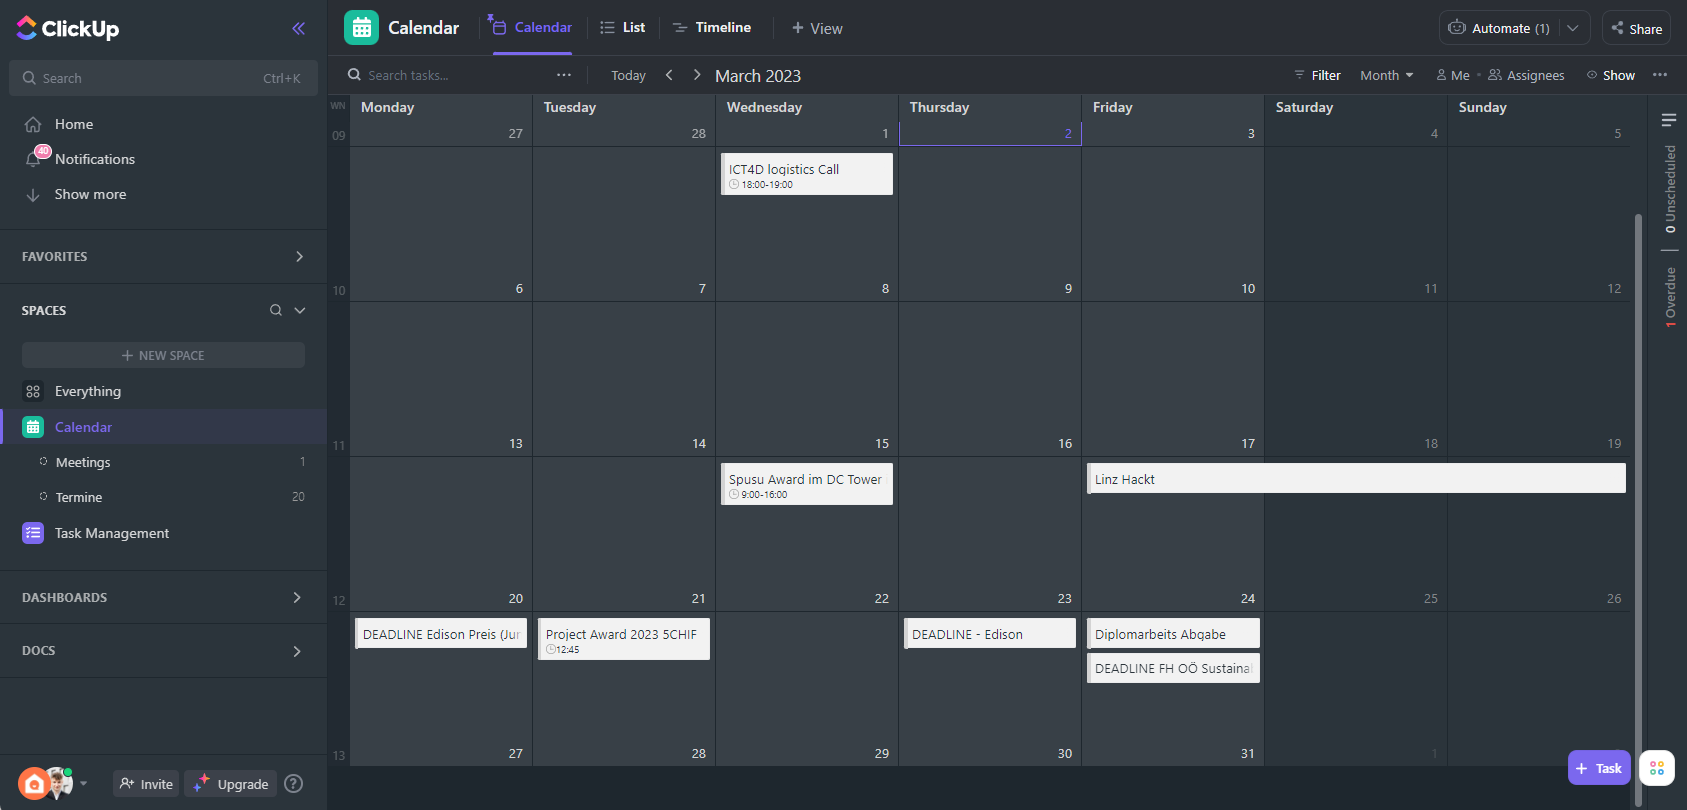
\includegraphics[width=1\textwidth]{./pics/clickup-calender-view.png}
    \caption{ClickUp Dashboard Kalender}
    \label{fig:clickup-calendar}
\end{figure}


In der Diplomarbeit wurden viele Mentoring-Sessions, Meetings mit dem Diplomarbeitbetreuer und weitere Termine wie Wettbewerbe vereinbart. Ohne eine geeignete Methode zur Verwaltung all dieser Termine kann es schnell unübersichtlich werden. Deshalb wurde das Kalender-Feature von ClickUp genutzt, um alle Einträge abzubilden, wie in Abbildung \ref{fig:clickup-calendar} zu sehen ist. Der Kalender wurde automatisch mit den persönlichen Kalendern synchronisiert, wie beispielsweise einem Google Kalender. Dadurch wurden nie Termine verpasst, was insbesondere dem Projektleiter sehr geholfen hat, da er nicht jeden daran erinnern musste, alle Termine in seinem Kalender einzutragen.

Ein weiterer wichtiger Punkt war das Task-Management in dem Projekt. Da im Projekt schnell viele Aufgaben koordiniert werden mussten, war es sinnvoll, alle Aufgaben in einer simplen To-Do-Liste abzubilden. Vor den Semesterferien wurde beispielsweise eine eigene Abteilung für Ferien-Tasks erstellt, um einen Überblick über alle Aufgaben während der Semesterferien zu haben. Obwohl die Tasks-To-Listen nicht aktiv genutzt wurden, war es sehr praktisch, um den Fortschritt zu überwachen und sicherzustellen, dass alles rechtzeitig erledigt wurde.

Zusammenfassend war ClickUp eine große Bereicherung für das
Projektmanagement, da es viel Zeit bei der Verwaltung von
Terminen und Aufgaben gespart hat. Auch die Benutzung als
neuer Benutzer war sehr einfach, sodass keine lange
Einarbeitungszeit nötig war. Besonders faszinierend ist,
dass ClickUp sehr intuitiv ist und viele nützliche Features
bietet.

